%% ===========================================================================
\FloatBarrier
\section{Formulation}
\label{sec:formulation}
%% ===========================================================================

The model is a two-dimensional electromechanical continuum with three
enrichments: the strain-gradient energy is generated by the second moment of a
rectangular nonlocal averaging window, the electric enthalpy carries the
piezoelectric and the flexoelectric couplings together, and the dielectric
response is a fractional Kelvin--Voigt law. The derivation below follows the
order in which the finite element needs the result -- window, kinematics,
energy, constitutive relations, reduction, memory, governing equations -- and
the closed-form window coefficients are collected in \ref{app:Mcoeff}.

\FloatBarrier
\subsection{Nonlocal averaging window and the second-moment tensor}
\label{sec:window}

Let the strain gradient at a material point $\bm{x}$ be replaced by its average
over a window $\mathcal{W}$ of area $A_{\mathcal W}$ centred at that point,
\begin{equation}
  \bar\eta_{ijk}(\bm{x}) = \frac{1}{A_{\mathcal W}}
     \int_{\mathcal W} \eta_{ijk}(\bm{x}+\bm{s})\,\mathrm{d}\bm{s}.
  \label{eq:average}
\end{equation}
Expanding the integrand to second order in the window coordinate,
\begin{equation}
  \eta_{ijk}(\bm{x}+\bm{s}) \simeq \eta_{ijk}(\bm{x})
     + s_m\,\eta_{ijk,m}(\bm{x}) + \tfrac12 s_m s_n\,\eta_{ijk,mn}(\bm{x}),
  \label{eq:expand}
\end{equation}
and integrating term by term, the linear term vanishes because the window is
centred, so
\begin{equation}
  \bar\eta_{ijk} \simeq \eta_{ijk} + \tfrac12 M_{mn}\,\eta_{ijk,mn},
  \qquad
  M_{mn} = \frac{1}{A_{\mathcal W}}\int_{\mathcal W} s_m s_n \,\mathrm{d}\bm{s},
  \label{eq:Mdef}
\end{equation}
and every geometric property of the window enters the model through the
symmetric second-order tensor $M$, which has the dimensions of a squared
length and plays the role that a scalar characteristic length plays in
isotropic strain-gradient elasticity. For the three windows used in this work
the diagonal components follow from elementary integration,
\begin{equation}
  M^{\rm cuboid}_{ii} = \frac{a_i^2}{3},\qquad
  M^{\rm ellipse}_{ii} = \frac{a_i^2}{4},\qquad
  M^{\rm ellipsoid}_{ii} = \frac{a_i^2}{5},
  \label{eq:Mshapes}
\end{equation}
where $a_i$ are the half-widths in two dimensions and the semi-axes in three.
A window rotated by $\theta$ in the plane is obtained from the axis-aligned
tensor by $M\mapsto RMR^{\mathsf T}$, that is
\begin{equation}
  M_{11}(\theta)=M_{11}\cos^{2}\theta+M_{22}\sin^{2}\theta,\qquad
  M_{12}(\theta)=\tfrac12\left(M_{22}-M_{11}\right)\sin2\theta,
  \label{eq:Mrot2}
\end{equation}
so the off-diagonal component grows with $\sin2\theta$ and the diagonal ones
carry the orientation dependence.

Equation~\eqref{eq:Mshapes} has a consequence that is used throughout the
paper and is verified in Sec.~\ref{sec:windowshape}: once $M$ is fixed the
\emph{shape} of the window carries no information, because two windows with the
same second moment produce identical solutions. The shape is therefore not a
free parameter of the model, whereas the anisotropy of the window -- its aspect
ratio and its orientation -- is a genuine material-geometry parameter, since it
changes $M$ and with it the ratio between the directional gradient penalties.

\FloatBarrier
\subsection{Kinematics}
\label{sec:kinematics}

Let $\Omega\subset\mathbb{R}^2$ be the mid-plane of a strip of thickness $h$,
with coordinates $x_1$ along the member and $x_2$ through its thickness. The
mechanical state is the pair $(u_1,u_2)$, where $u_1$ is the in-plane
displacement and $u_2\equiv w$ is the transverse deflection, the model retains
the full second gradient of both components, and the strain and the strain
gradient are
\begin{equation}
  \varepsilon_{ij} = \tfrac12\left(u_{i,j}+u_{j,i}\right),\qquad
  \eta_{ijk} = \partial_k \varepsilon_{ij} = \tfrac12\left(
  u_{i,jk}+u_{j,ik}\right),
  \label{eq:strain}
\end{equation}
so that the mechanical degrees of freedom at a node are the eight quantities
\begin{equation}
  \left\{u_1,\; \partial_1u_1,\; \partial_2u_1,\; \partial_{12}u_1,\;
         u_2,\; \partial_1u_2,\; \partial_2u_2,\; \partial_{12}u_2\right\},
  \label{eq:dofs}
\end{equation}
that is, the value, the two first derivatives and the cross derivative of each
component -- eight mechanical degrees of freedom per node and not a
three-component continuum. These are the degrees of freedom of the
Bogner--Fox--Schmit rectangle~\cite{BognerFoxSchmit1966}: a bicubic Hermite
tensor-product element, $C^1$ across element edges and $C^0$ only for the
cross derivative, in which the displacement of one component is interpolated
from its nodal data as
\begin{equation}
  u(\xi,\eta) = \sum_{a=1}^{4}\Big[N^{00}_{a}u_a + N^{10}_{a}u_{,x}\big|_a
    + N^{01}_{a}u_{,y}\big|_a + N^{11}_{a}u_{,xy}\big|_a\Big],
  \label{eq:interp}
\end{equation}
with $N^{pq}_a$ the products of the one-dimensional Hermite cubics. It is the
natural carrier of $\eta_{ijk}$ in two dimensions and it is the element family
used in the one-scale theory~\cite{fem1}; here it is extended by the
flexoelectric and fractional-memory terms rather than replaced.

\FloatBarrier
\subsection{Electric enthalpy and the piezoelectric--flexoelectric
constitutive relations}
\label{sec:energy}

The electromechanical enthalpy of the strip is assembled from five terms. The
elastic energy is
\begin{equation}
  \Pi_{\rm el} = \tfrac12\int_\Omega \varepsilon_{ij} C_{ijkl}
        \varepsilon_{kl}\,\mathrm{d}A ,
  \label{eq:Eel}
\end{equation}
the gradient energy is the window average of the elastic energy truncated at
the second moment, which by \eqref{eq:Mdef} is
\begin{equation}
  \Pi_{\rm gr} = \tfrac14\int_\Omega M_{mn}\,
        \varepsilon_{ij,m}\,C_{ijkl}\,\varepsilon_{kl,n}\,\mathrm{d}A ,
  \label{eq:Egrad}
\end{equation}
the piezoelectric and dielectric energies are
\begin{equation}
  \Pi_{\rm pz} = -\int_\Omega e_{kij} E_k \varepsilon_{ij}\,\mathrm{d}A
  \qquad\text{and}\qquad
  \Pi_{\rm dl} = -\tfrac12\int_\Omega \kappa_{ij} E_i E_j\,\mathrm{d}A ,
  \label{eq:Epiezo}
\end{equation}
and the flexoelectric term is the polarization-gradient coupling of Mindlin's
Form~II~\cite{Mindlin1965,Toupin1962,Mindlin1968},
\begin{equation}
  \Pi_{\rm fx} = -\int_\Omega \mu_{kijl} E_k \eta_{ijl}\,\mathrm{d}A ,
  \label{eq:Eflexo}
\end{equation}
where $E_k=-\phi_{,k}$ is the electric field, $\phi$ the electric potential,
$C_{ijkl}$ the elastic stiffness, $e_{kij}$ the piezoelectric tensor,
$\kappa_{ij}$ the permittivity, $\mu_{kijl}$ the flexoelectric tensor,
$\eta_{ijl}=\varepsilon_{ij,l}$ the strain gradient of \eqref{eq:strain},
$M_{mn}$ the second moment of the averaging window and $W_{\rm ext}$ the work
of the external loads. The total enthalpy is their sum,
\begin{equation}
  \Pi = \Pi_{\rm el} + \Pi_{\rm gr} + \Pi_{\rm pz} + \Pi_{\rm dl}
        + \Pi_{\rm fx} - W_{\rm ext},
  \label{eq:energy}
\end{equation}
in which the isotropic length $\ell^2\delta_{mn}$ of a scalar theory is
replaced by $M_{mn}$ in \eqref{eq:Egrad}. The flexoelectric tensor is taken
isotropic and is represented by the single coefficient
\begin{equation}
  \mu_{kijl} = \mu\,\delta_{ij}\delta_{kl},
  \qquad \mu = 10^{-6}\ \si{\coulomb\per\metre},
  \label{eq:muexplicit}
\end{equation}
a charge per unit length, so every flexoelectric energy in this paper scales as
$\mu$ and every flexoelectric coupling as $\mu^{2}$.

The constitutive relations are the derivatives of $\Pi$ with respect to the
three kinematic variables. The stress is
\begin{equation}
  \sigma_{ij} = \frac{\partial \Pi}{\partial \varepsilon_{ij}}
              = C_{ijkl}\,\varepsilon_{kl} - e_{kij} E_k ,
  \label{eq:sig}
\end{equation}
the higher-order stress is
\begin{equation}
  \varsigma_{ijm} = \frac{\partial \Pi}{\partial \varepsilon_{ij,m}}
              = \tfrac12 M_{mn}\,C_{ijkl}\,\varepsilon_{kl,n}
                - \mu_{kijm}\,E_k ,
  \label{eq:tau}
\end{equation}
and the electric displacement is
\begin{equation}
  D_k = -\frac{\partial \Pi}{\partial E_k}
              = e_{kij}\,\varepsilon_{ij} + \kappa_{kl}\,E_l
                + \mu_{kijl}\,\eta_{ijl},
  \label{eq:D}
\end{equation}
so that the electric displacement contains the strain, the field and the strain
gradient, while the higher-order stress $\varsigma_{ijm}$ is not an
independent constitutive object but the elastic stress transported through the
window. With the single-constant tensor \eqref{eq:muexplicit} the last two
relations become
\begin{equation}
  \varsigma_{ijm} = \tfrac12 M_{mn}\,C_{ijkl}\,\varepsilon_{kl,n}
                    - \mu E_m\delta_{ij},
  \qquad
  D_k = e_{kij}\varepsilon_{ij} + \kappa_{kl}E_l
        + \mu\,\partial_k\left(\varepsilon_{xx}+\varepsilon_{yy}\right),
  \label{eq:Dexplicit}
\end{equation}
which is the form the element assembles. An ellipsoidal window carries
$M_{mn}=L_{mn}/5$ in the notation of the one-scale theory with a tensorial
characteristic length, so $\tfrac14 M_{mn}=\tfrac1{20}L_{mn}$ and the gradient
energy of~\cite{fem1} is recovered exactly.

The three relations are derivatives of the one enthalpy \eqref{eq:energy} taken
with $E_k=-\phi_{,k}$, and their signs are those of the implementation: the
dielectric energy enters $\Pi$ with a minus sign so that $D$ carries
$+\kappa_{kl}E_l$, the assembled dielectric block is
$K_{\phi\phi}=+\int\nabla N_\phi^{\mathsf T}\kappa\nabla N_\phi$, the
piezoelectric coupling is $B=\int B^{\mathsf T}e^{\mathsf T}\nabla N_\phi$, and
the flexoelectric coupling $+\int\mu\,\nabla N_\phi^{\mathsf T}
\nabla(\varepsilon_{xx}+\varepsilon_{yy})$ is carried by the same gradient of
the potential. A sign error in any one of the three would show up as an
asymmetry between $B$ and $B^{\mathsf T}$ rather than as a change of a number.

The second term of \eqref{eq:energy} is the second-moment truncation of the
window average of the elastic energy and not an asymptotic expansion of it:
Taylor expanding the strain about the centroid of the window and averaging
with $\langle s_m\rangle=0$, $\langle s_ms_n\rangle=M_{mn}$ leaves a quadratic
functional in the strain gradient whose kernel is the second-moment tensor, so
the coefficient of the gradient energy is fixed by the window and is not a
fitted length. The truncation is exact for a strain that varies affinely across
the window and is in error at the next order in $a_i\partial\varepsilon$; its
adequacy has to be established for the material at hand
(Sec.~\ref{sec:limit_window}) rather than assumed from a convergent series.

Three remarks on \eqref{eq:energy} matter for the implementation. First, the
gradient term couples the third derivatives of the displacement, so the element
must be $C^1$ in the sense of \eqref{eq:dofs}; a $C^0$ element would make the
fourth-order term non-conforming. Second, the piezoelectric and flexoelectric
couplings appear in the same enthalpy but not in the same devices: they are
collected by different electrode pairs, as Sec.~\ref{sec:bc} makes explicit.
Third, because the strip is treated as a two-dimensional continuum, the
plane-stress or plane-strain reduction of $C$, $e$ and $\kappa$ is part of the
model rather than a detail of the implementation.

\FloatBarrier
\subsection{Two-dimensional reduction of the material tensors}
\label{sec:reduction}

The strip is free out of plane, so the stress component normal to the plane
vanishes and the stiffness that multiplies the in-plane strain is the reduced
tensor
\begin{equation}
  C^{p}_{ij} = C_{ij} - \frac{C_{i3}C_{j3}}{C_{33}},
  \label{eq:Cp}
\end{equation}
with the corresponding reductions of the piezoelectric and dielectric tensors,
\begin{equation}
  e^{p}_{ij} = e_{ij} - \frac{C_{i3}}{C_{33}}\,e_{3j},
  \qquad
  \kappa^{p}_{ij} = \kappa_{ij} + \frac{e_{3i}e_{3j}}{C_{33}},
  \label{eq:ep}
\end{equation}
while the plane-strain alternative keeps $C$ and drops the out-of-plane strain
instead. The two reductions are not interchangeable: for the strip of
Table~\ref{tab:params}, poled along the length, the plane-stress entry is
$C^{p}_{xx}=9.5500\times10^{10}$\,Pa against $C_{xx}=2.22\times10^{11}$\,Pa in
plane strain, and the extensional coupling factor of the two is $0.5581$ and
$0.5132$ respectively. The plane-stress reduction is used everywhere below
because the strip is free out of plane, and the difference between the two is
reported in Sec.~\ref{sec:verification}.

\FloatBarrier
\subsection{Fractional Kelvin--Voigt memory}
\label{sec:fracmem}

The dielectric relaxation is described by a fractional Kelvin--Voigt element in
which the quantity conjugate to the electric field carries a Caputo derivative
of order $\alpha$. The Caputo derivative of a function that starts from rest
is
\begin{equation}
  {}^{C}\!D_t^{\alpha}f(t) = \frac{1}{\Gamma(1-\alpha)}
     \int_{0}^{t}\frac{\dot f(t')}{(t-t')^{\alpha}}\,\mathrm{d}t',
  \qquad 0<\alpha\le1,
  \label{eq:caputo}
\end{equation}
and the spring-pot of Caputo~\cite{Caputo1967}, whose use as a constitutive
element is due to Bagley and Torvik~\cite{BagleyTorvik1983} and
Koeller~\cite{Koeller1984}, is
\begin{equation}
  \sigma(t) = K\,\varepsilon(t) + K\,\tau^{\alpha}\,
              {}^{C}\!D_t^{\alpha}\varepsilon(t),
  \label{eq:kv}
\end{equation}
with $\tau$ a relaxation time and $K$ the appropriate stiffness. The model is
the fractional counterpart of the Cole--Cole description of a broadened
dielectric relaxation~\cite{ColeCole1941,HavriliakNegami1967}, and its
frequency-domain modulus,
\begin{equation}
  K^{*}(\omega) = K\left[1+(\mathrm{i}\omega\tau)^{\alpha}\right],
  \label{eq:kvfreq}
\end{equation}
reduces to the classical Kelvin--Voigt element for $\alpha=1$.

Two matrices are candidates for the $K$ of \eqref{eq:kv} in the condensed
mechanical problem: the fully condensed stiffness $K_{\rm eff}$, which
contains the electrical boundary condition, and the short-circuit stiffness
$K_{uu}$, which does not. They are different models of the same physics, not
two numerical conventions, and Sec.~\ref{sec:memorystudy} quantifies the
difference. Discretising \eqref{eq:caputo} with the L1 scheme at uniform steps
$\Delta t$ gives
\begin{equation}
  {}^{C}\!D_t^{\alpha}\varepsilon(t_n) \approx
  \frac{1}{\Gamma(2-\alpha)}\sum_{k=1}^{n} b_{n-k}\,
  \frac{\varepsilon^{k}-\varepsilon^{k-1}}{\Delta t^{\alpha}},
  \label{eq:l1}
\end{equation}
with the weights
\begin{equation}
  b_j=(j+1)^{1-\alpha}-j^{1-\alpha},\qquad b_0=1,
  \label{eq:bdef}
\end{equation}
computed once for the whole history and reused at every step. Two properties of
the weights are used below: they decay algebraically, so the history is never
forgotten, and at $\alpha=1$ they collapse to $b_0=1$, $b_j=0$ for $j\ge1$, so
that the scheme becomes a backward difference and the memory reduces to the
classical Kelvin--Voigt law up to its first-order truncation error. The
convolution is applied to the reduced modal coordinates, so the history that
has to be stored is one scalar sequence per retained mode and the cost per step
does not grow with the number of elements; which of the two matrices enters
\eqref{eq:kv} decides whether the piezoelectric contribution is inside the
remembered operator or outside it. The L1 discretization is first order in time
for every order $\alpha\in(0,1]$, at $\alpha=1$ as well, because the newest
increment enters through a backward difference; the sequence that measures the
order, and the step the results use, are reported in Sec.~\ref{sec:verification}.

\FloatBarrier
\subsection{Governing equations}
\label{sec:governing}

Stationarity of \eqref{eq:energy} with respect to the mechanical field and to
the potential gives the strong form on $\Omega$,
\begin{align}
  \sigma_{ij,j} - \varsigma_{ijm,jm} + \rho\,\ddot u_i &= 0,
  \label{eq:gov1}\\
  D_{k,k} &= 0,
  \label{eq:gov2}
\end{align}
together with the classical traction and the higher-order double-traction
conditions on the boundary, which are stated in Sec.~\ref{sec:bc}. With
\eqref{eq:Dexplicit} substituted, the two equations read
\begin{equation}
  \left(C_{ijkl}\varepsilon_{kl}\right)_{,j}
    - \left[\tfrac12 M_{mn}C_{ijkl}\varepsilon_{kl,n}\right]_{,jm}
    + \mu\left(\nabla\cdot\bm{E}\right)_{,i} + \rho\ddot u_i = 0,
  \qquad
  \kappa_{kl}E_{l,k} = -\mu\,\partial_k\partial_k
    \left(\varepsilon_{xx}+\varepsilon_{yy}\right),
  \label{eq:govexp}
\end{equation}
so that \eqref{eq:gov1} carries the flexoelectric term
$\mu(\nabla\cdot\bm E)_{,i}$ and \eqref{eq:gov2} carries
$\mu\partial_k\partial_k(\varepsilon_{xx}+\varepsilon_{yy})$; the two are the
transpose pair that the weak form assembles. The mechanical boundary condition
of the gradient theory is the pair $(t_i,\,m_i)$ -- force and double force per
unit length -- so a clamped edge constrains both the displacement and its
normal derivative, exactly the quantities that appear in \eqref{eq:dofs}. In
the time domain the memory of \eqref{eq:kv} turns \eqref{eq:gov1} into a
Volterra-type equation whose kernel is the fractional derivative of
\eqref{eq:l1}; the weak form of Sec.~\ref{sec:fem} is written directly for the
time-discrete problem, which is what the implementation solves.

Three effects enter at this point and are kept apart throughout: the memory of
\eqref{eq:kv} acts on the \emph{damping} at fixed eigenfrequency, the window of
\eqref{eq:Mdef} acts on the \emph{stiffness} at fixed memory, and the
flexoelectric tensor $\mu$ acts on the \emph{coupling} at fixed geometry. No
result below is attributed to one of them when it was computed with another
changed.

The two electrode arrangements referred to throughout the paper are fixed in
Fig.~\ref{fig:geometry}: the bending family is poled across the thickness with
electrodes on the long faces, and the extensional family is poled along the
length with electrodes on the end faces. They are two electrical
configurations of one strip, and the coupling factors obtained from them are
therefore not additive.

The parameters of the model are collected in Table~\ref{tab:params}. The
elastic, piezoelectric and dielectric constants are the values measured by
Zgonik and co-workers for $\mathrm{BaTiO_3}$~\cite{Zgonik1994}; the mass
density is the standard crystallographic value for the same material. Five
quantities are assumed rather than measured, and they are listed in the same
table: the flexoelectric coefficient, taken as
$\mu=10^{-6}$\,\si{\coulomb\per\metre}, which is the order reported for
perovskite ceramics, so that every flexoelectric coupling below is to be read
as scaling with $\mu^{2}$; the window half-widths, which are held at
$a_1/L\le0.2$ as the operating range of the second-moment truncation assumes;
the fractional order and the relaxation time, which are free parameters of the
memory law and are varied over the ranges stated; and the mesh, which the
convergence study of Sec.~\ref{sec:verification} shows to be adequate for
every quantity quoted.

%% The parameter table: quantity, symbol, value, unit.  The source of every
%% value is stated in the sentence above the table, not in a column.
\begin{table}[!t]
\centering
\small
\caption{Parameters of the model. The sources of the first four rows are given
in the text above the table; the five rows below the rule are assumed and their
effect is stated there and in Secs.~\ref{sec:material} and
\ref{sec:limitations}.}
\label{tab:params}
\begin{tabular}{@{}llll@{}}
\toprule
quantity & symbol & value & unit \\
\midrule
elastic constants & $C_{11}$, $C_{12}$, $C_{13}$, $C_{33}$, $C_{44}$ &
$222$, $108$, $111$, $151$, $61$ & GPa \\
piezoelectric constants & $e_{15}$, $e_{31}$, $e_{33}$ &
$34.2$, $-0.7$, $6.7$ & \si{\coulomb\per\square\metre} \\
relative permittivities & $\kappa_{11}/\kappa_0$, $\kappa_{33}/\kappa_0$ &
$2200$, $56$ & -- \\
mass density & $\rho$ & $6020$ & \si{\kilo\gram\per\cubic\metre} \\
\midrule
flexoelectric coefficient & $\mu$ & $10^{-6}$ & \si{\coulomb\per\metre} \\
window half-widths & $a_1$, $a_2$ & $3$, $1$ & \si{\micro\metre} \\
fractional order & $\alpha$ & $0.5$--$1$ & -- \\
relaxation time & $\tau$ & $0.3$--$30$ & \si{\nano\second} \\
strip geometry & $L$, $h$ & $200$, $10$ & \si{\micro\metre} \\
mesh & -- & $48\times4$ BFS elements & -- \\
\bottomrule
\end{tabular}
\end{table}


\begin{figure}[!t]
\centering
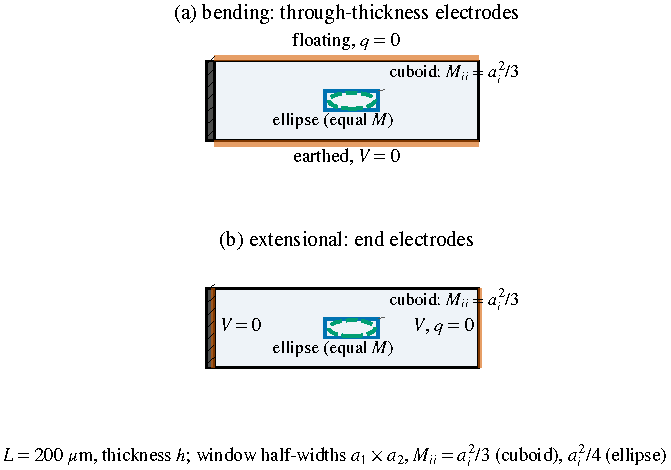
\includegraphics[width=\textwidth]{F1_geometry.pdf}
\caption{The two electrode configurations and the averaging window.
(a) Bending family, poled through the thickness: electrodes on the large
faces, the lower earthed and the upper floating at zero net charge.
(b) Extensional family, poled along the length: electrodes on the short ends.
The window is a rectangle of half-widths $a_1\times a_2$, whose second moment
fixes the gradient energy.}
\label{fig:geometry}
\end{figure}

\FloatBarrier
